\documentclass[tikz]{standalone}
\begin{document}
	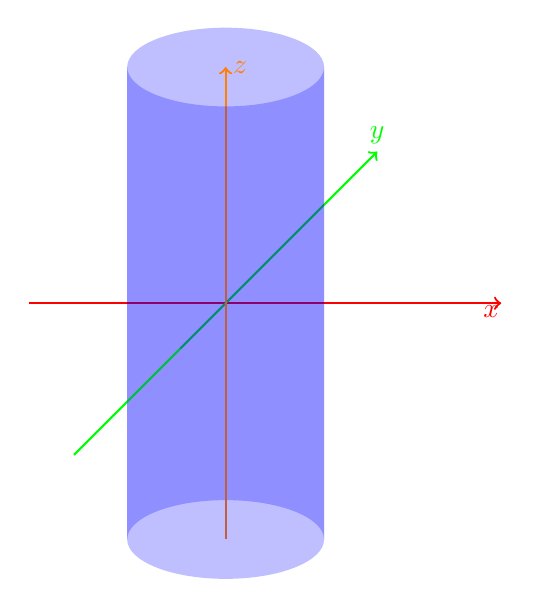
\begin{tikzpicture}
		
		\draw[red,thick, ->] (-2.5,0,0) -- (3.5,0,0) node[below left=-3]{$x$};
		\draw[green,thick, ->] (0,0,1.5) -- (0,0,-5) node[above=-1]{$y$};	
		
		\fill [blue, nearly transparent] (1.25,-3) -- (1.25, 3) arc (0:180:1.25 and 0.5) -- (-1.25,-3) arc (180:360:1.25 and -0.5);
		\draw[green, thick] (0,0,5) -- (0,0,1.5);
		\draw[orange, thick, ->] (0,-3,0) -- (0,3,0) node[right=-1]{$z$};
		
		\fill [blue, nearly transparent] (-1.25,-3) -- (-1.25, 3) arc (180:360:1.25 and 0.5) -- (1.25,-3) arc (0:180:1.25 and -0.5);		
		
	\end{tikzpicture}
\end{document}